% Options for packages loaded elsewhere
\PassOptionsToPackage{unicode}{hyperref}
\PassOptionsToPackage{hyphens}{url}
\PassOptionsToPackage{dvipsnames,svgnames,x11names}{xcolor}
%
\documentclass[
  letterpaper,
  DIV=11,
  numbers=noendperiod]{scrartcl}

\usepackage{amsmath,amssymb}
\usepackage{iftex}
\ifPDFTeX
  \usepackage[T1]{fontenc}
  \usepackage[utf8]{inputenc}
  \usepackage{textcomp} % provide euro and other symbols
\else % if luatex or xetex
  \usepackage{unicode-math}
  \defaultfontfeatures{Scale=MatchLowercase}
  \defaultfontfeatures[\rmfamily]{Ligatures=TeX,Scale=1}
\fi
\usepackage{lmodern}
\ifPDFTeX\else  
    % xetex/luatex font selection
\fi
% Use upquote if available, for straight quotes in verbatim environments
\IfFileExists{upquote.sty}{\usepackage{upquote}}{}
\IfFileExists{microtype.sty}{% use microtype if available
  \usepackage[]{microtype}
  \UseMicrotypeSet[protrusion]{basicmath} % disable protrusion for tt fonts
}{}
\makeatletter
\@ifundefined{KOMAClassName}{% if non-KOMA class
  \IfFileExists{parskip.sty}{%
    \usepackage{parskip}
  }{% else
    \setlength{\parindent}{0pt}
    \setlength{\parskip}{6pt plus 2pt minus 1pt}}
}{% if KOMA class
  \KOMAoptions{parskip=half}}
\makeatother
\usepackage{xcolor}
\setlength{\emergencystretch}{3em} % prevent overfull lines
\setcounter{secnumdepth}{5}
% Make \paragraph and \subparagraph free-standing
\ifx\paragraph\undefined\else
  \let\oldparagraph\paragraph
  \renewcommand{\paragraph}[1]{\oldparagraph{#1}\mbox{}}
\fi
\ifx\subparagraph\undefined\else
  \let\oldsubparagraph\subparagraph
  \renewcommand{\subparagraph}[1]{\oldsubparagraph{#1}\mbox{}}
\fi

\usepackage{color}
\usepackage{fancyvrb}
\newcommand{\VerbBar}{|}
\newcommand{\VERB}{\Verb[commandchars=\\\{\}]}
\DefineVerbatimEnvironment{Highlighting}{Verbatim}{commandchars=\\\{\}}
% Add ',fontsize=\small' for more characters per line
\usepackage{framed}
\definecolor{shadecolor}{RGB}{241,243,245}
\newenvironment{Shaded}{\begin{snugshade}}{\end{snugshade}}
\newcommand{\AlertTok}[1]{\textcolor[rgb]{0.68,0.00,0.00}{#1}}
\newcommand{\AnnotationTok}[1]{\textcolor[rgb]{0.37,0.37,0.37}{#1}}
\newcommand{\AttributeTok}[1]{\textcolor[rgb]{0.40,0.45,0.13}{#1}}
\newcommand{\BaseNTok}[1]{\textcolor[rgb]{0.68,0.00,0.00}{#1}}
\newcommand{\BuiltInTok}[1]{\textcolor[rgb]{0.00,0.23,0.31}{#1}}
\newcommand{\CharTok}[1]{\textcolor[rgb]{0.13,0.47,0.30}{#1}}
\newcommand{\CommentTok}[1]{\textcolor[rgb]{0.37,0.37,0.37}{#1}}
\newcommand{\CommentVarTok}[1]{\textcolor[rgb]{0.37,0.37,0.37}{\textit{#1}}}
\newcommand{\ConstantTok}[1]{\textcolor[rgb]{0.56,0.35,0.01}{#1}}
\newcommand{\ControlFlowTok}[1]{\textcolor[rgb]{0.00,0.23,0.31}{#1}}
\newcommand{\DataTypeTok}[1]{\textcolor[rgb]{0.68,0.00,0.00}{#1}}
\newcommand{\DecValTok}[1]{\textcolor[rgb]{0.68,0.00,0.00}{#1}}
\newcommand{\DocumentationTok}[1]{\textcolor[rgb]{0.37,0.37,0.37}{\textit{#1}}}
\newcommand{\ErrorTok}[1]{\textcolor[rgb]{0.68,0.00,0.00}{#1}}
\newcommand{\ExtensionTok}[1]{\textcolor[rgb]{0.00,0.23,0.31}{#1}}
\newcommand{\FloatTok}[1]{\textcolor[rgb]{0.68,0.00,0.00}{#1}}
\newcommand{\FunctionTok}[1]{\textcolor[rgb]{0.28,0.35,0.67}{#1}}
\newcommand{\ImportTok}[1]{\textcolor[rgb]{0.00,0.46,0.62}{#1}}
\newcommand{\InformationTok}[1]{\textcolor[rgb]{0.37,0.37,0.37}{#1}}
\newcommand{\KeywordTok}[1]{\textcolor[rgb]{0.00,0.23,0.31}{#1}}
\newcommand{\NormalTok}[1]{\textcolor[rgb]{0.00,0.23,0.31}{#1}}
\newcommand{\OperatorTok}[1]{\textcolor[rgb]{0.37,0.37,0.37}{#1}}
\newcommand{\OtherTok}[1]{\textcolor[rgb]{0.00,0.23,0.31}{#1}}
\newcommand{\PreprocessorTok}[1]{\textcolor[rgb]{0.68,0.00,0.00}{#1}}
\newcommand{\RegionMarkerTok}[1]{\textcolor[rgb]{0.00,0.23,0.31}{#1}}
\newcommand{\SpecialCharTok}[1]{\textcolor[rgb]{0.37,0.37,0.37}{#1}}
\newcommand{\SpecialStringTok}[1]{\textcolor[rgb]{0.13,0.47,0.30}{#1}}
\newcommand{\StringTok}[1]{\textcolor[rgb]{0.13,0.47,0.30}{#1}}
\newcommand{\VariableTok}[1]{\textcolor[rgb]{0.07,0.07,0.07}{#1}}
\newcommand{\VerbatimStringTok}[1]{\textcolor[rgb]{0.13,0.47,0.30}{#1}}
\newcommand{\WarningTok}[1]{\textcolor[rgb]{0.37,0.37,0.37}{\textit{#1}}}

\providecommand{\tightlist}{%
  \setlength{\itemsep}{0pt}\setlength{\parskip}{0pt}}\usepackage{longtable,booktabs,array}
\usepackage{calc} % for calculating minipage widths
% Correct order of tables after \paragraph or \subparagraph
\usepackage{etoolbox}
\makeatletter
\patchcmd\longtable{\par}{\if@noskipsec\mbox{}\fi\par}{}{}
\makeatother
% Allow footnotes in longtable head/foot
\IfFileExists{footnotehyper.sty}{\usepackage{footnotehyper}}{\usepackage{footnote}}
\makesavenoteenv{longtable}
\usepackage{graphicx}
\makeatletter
\def\maxwidth{\ifdim\Gin@nat@width>\linewidth\linewidth\else\Gin@nat@width\fi}
\def\maxheight{\ifdim\Gin@nat@height>\textheight\textheight\else\Gin@nat@height\fi}
\makeatother
% Scale images if necessary, so that they will not overflow the page
% margins by default, and it is still possible to overwrite the defaults
% using explicit options in \includegraphics[width, height, ...]{}
\setkeys{Gin}{width=\maxwidth,height=\maxheight,keepaspectratio}
% Set default figure placement to htbp
\makeatletter
\def\fps@figure{htbp}
\makeatother

\usepackage{fvextra}
\DefineVerbatimEnvironment{Highlighting}{Verbatim}{breaklines,commandchars=\\\{\}}
\DefineVerbatimEnvironment{OutputCode}{Verbatim}{breaklines,commandchars=\\\{\}}
\KOMAoption{captions}{tableheading}
\makeatletter
\makeatother
\makeatletter
\makeatother
\makeatletter
\@ifpackageloaded{caption}{}{\usepackage{caption}}
\AtBeginDocument{%
\ifdefined\contentsname
  \renewcommand*\contentsname{Table of contents}
\else
  \newcommand\contentsname{Table of contents}
\fi
\ifdefined\listfigurename
  \renewcommand*\listfigurename{List of Figures}
\else
  \newcommand\listfigurename{List of Figures}
\fi
\ifdefined\listtablename
  \renewcommand*\listtablename{List of Tables}
\else
  \newcommand\listtablename{List of Tables}
\fi
\ifdefined\figurename
  \renewcommand*\figurename{Figure}
\else
  \newcommand\figurename{Figure}
\fi
\ifdefined\tablename
  \renewcommand*\tablename{Table}
\else
  \newcommand\tablename{Table}
\fi
}
\@ifpackageloaded{float}{}{\usepackage{float}}
\floatstyle{ruled}
\@ifundefined{c@chapter}{\newfloat{codelisting}{h}{lop}}{\newfloat{codelisting}{h}{lop}[chapter]}
\floatname{codelisting}{Listing}
\newcommand*\listoflistings{\listof{codelisting}{List of Listings}}
\makeatother
\makeatletter
\@ifpackageloaded{caption}{}{\usepackage{caption}}
\@ifpackageloaded{subcaption}{}{\usepackage{subcaption}}
\makeatother
\makeatletter
\@ifpackageloaded{tcolorbox}{}{\usepackage[skins,breakable]{tcolorbox}}
\makeatother
\makeatletter
\@ifundefined{shadecolor}{\definecolor{shadecolor}{rgb}{.97, .97, .97}}
\makeatother
\makeatletter
\makeatother
\makeatletter
\makeatother
\ifLuaTeX
  \usepackage{selnolig}  % disable illegal ligatures
\fi
\IfFileExists{bookmark.sty}{\usepackage{bookmark}}{\usepackage{hyperref}}
\IfFileExists{xurl.sty}{\usepackage{xurl}}{} % add URL line breaks if available
\urlstyle{same} % disable monospaced font for URLs
\hypersetup{
  pdftitle={Automated MAIT cell annotation in Lett dataset using SingleR},
  pdfauthor={Ivan Osinnii},
  colorlinks=true,
  linkcolor={blue},
  filecolor={Maroon},
  citecolor={Blue},
  urlcolor={Blue},
  pdfcreator={LaTeX via pandoc}}

\title{Automated MAIT cell annotation in Lett dataset using SingleR}
\usepackage{etoolbox}
\makeatletter
\providecommand{\subtitle}[1]{% add subtitle to \maketitle
  \apptocmd{\@title}{\par {\large #1 \par}}{}{}
}
\makeatother
\subtitle{scRNA-seq workflow series part3}
\author{Ivan Osinnii}
\date{2024-04-18}

\begin{document}
\maketitle
\ifdefined\Shaded\renewenvironment{Shaded}{\begin{tcolorbox}[sharp corners, boxrule=0pt, breakable, enhanced, interior hidden, borderline west={3pt}{0pt}{shadecolor}, frame hidden]}{\end{tcolorbox}}\fi

\renewcommand*\contentsname{Table of contents}
{
\hypersetup{linkcolor=}
\setcounter{tocdepth}{3}
\tableofcontents
}
\hypertarget{introduction}{%
\section{Introduction}\label{introduction}}

In previous analyses we prepared our datasets in terms of data
normalization and UMAP projection. We also tried a simple case of MAIT
cell annotation taking well-annotated Garner et al.~dataset as a query
and MonacoImmuneData database as reference.

Here we take preprocessed data: both Lett experiment (liver cell subset)
and Garner et al.~dataset preprocessed and filtered (for liver tissue
and experiment 2). And we try to:\\
1) Project MonacoImmuneData MAIT cell labels on Lett dataset;\\
2) Project Garner et al.~dataset MAIT cell label on Lett dataset

In this way we want to be sure that if one of the methods shows some
result - it is not due to the batch effect and other types of artefacts,
or at least, it is not completely biased towards batch effect or
whatever else - donor variability etc.

Also, we want to make exact counts of MAIT cells in Lett dataset.

We start with loading data

\hypertarget{load-data-and-dependencies}{%
\section{Load data and dependencies}\label{load-data-and-dependencies}}

\begin{Shaded}
\begin{Highlighting}[]
\FunctionTok{library}\NormalTok{(SingleCellExperiment)}
\FunctionTok{library}\NormalTok{(SummarizedExperiment)}
\FunctionTok{library}\NormalTok{(Seurat)}
\FunctionTok{library}\NormalTok{(SingleR)}
\FunctionTok{library}\NormalTok{(pheatmap)}
\FunctionTok{library}\NormalTok{(ggplot2)}
\FunctionTok{library}\NormalTok{(RColorBrewer)}
\FunctionTok{library}\NormalTok{(tidyverse)}
\FunctionTok{library}\NormalTok{(scater)}
\FunctionTok{library}\NormalTok{(uwot)}
\FunctionTok{library}\NormalTok{(celldex)}
\end{Highlighting}
\end{Shaded}

\begin{Shaded}
\begin{Highlighting}[]
\NormalTok{lett.sce }\OtherTok{\textless{}{-}} \FunctionTok{readRDS}\NormalTok{(}\StringTok{"./input/Lett.sce.liver.gene.symbol\_analyzed.rds"}\NormalTok{)}
\NormalTok{lett.sce}
\end{Highlighting}
\end{Shaded}

\begin{verbatim}
class: SingleCellExperiment 
dim: 36169 6724 
metadata(3): Samples Samples Samples
assays(5): counts genefull spliced unspliced logcounts
rownames(36169): PLCXD1 LINC00685 ... '' ''
rowData names(12): GENEID SYMBOL ... max_prop_ambient topHVG
colnames(6724): BSSE_QGF_176995-AAACCCAAGACTCCGC
  BSSE_QGF_176995-AAACCCAAGATACAGT ... BSSE_QGF_176995-TTTGTTGCACACCGCA
  BSSE_QGF_176995-TTTGTTGTCGTTAGTG
colData names(23): Barcode SampleName ... MonImmCell label
reducedDimNames(7): PCA TSNE ... UMAP UMAP.2
mainExpName: RNA
altExpNames(0):
\end{verbatim}

\begin{Shaded}
\begin{Highlighting}[]
\NormalTok{lett.sce}\SpecialCharTok{$}\NormalTok{cellReferences\_celldex\_MonacoImmuneData }\OtherTok{\textless{}{-}}\NormalTok{ lett.sce}\SpecialCharTok{@}\NormalTok{colData}\SpecialCharTok{@}\NormalTok{listData[[}\StringTok{"cellReferences\_celldex\_MonacoImmuneData"}\NormalTok{]]}\SpecialCharTok{@}\NormalTok{listData[[}\StringTok{"labels"}\NormalTok{]]}
\FunctionTok{plotUMAP}\NormalTok{(lett.sce, }\AttributeTok{colour\_by =} \StringTok{\textquotesingle{}cellReferences\_celldex\_MonacoImmuneData\textquotesingle{}}\NormalTok{,}\AttributeTok{point\_size =} \FloatTok{1.0}\NormalTok{)}
\end{Highlighting}
\end{Shaded}

\begin{figure}[H]

{\centering 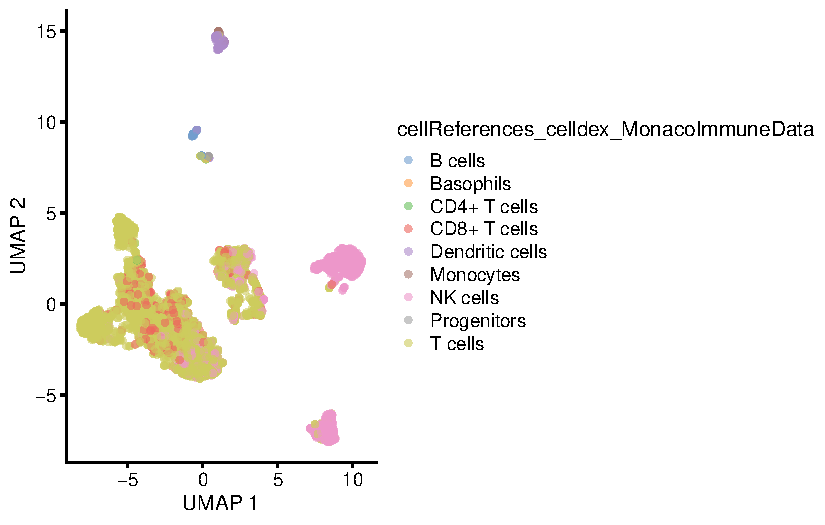
\includegraphics{2-Lett-data-SingleR_pdf_files/figure-pdf/unnamed-chunk-2-1.pdf}

}

\end{figure}

This UMAP was loaded into the Lett dataset by R. Ivanek and it shows
very general immune cell types like T cells, NK cells, B cells. We see
that our cells are mainly composed of these types in mentioned
order\ldots{}

\hypertarget{analysis-with-singler-and-monacoimmunedata-reference}{%
\section{Analysis with SingleR and MonacoImmuneData
reference}\label{analysis-with-singler-and-monacoimmunedata-reference}}

Extract count matrix from sce object for query data and load reference

\begin{Shaded}
\begin{Highlighting}[]
\NormalTok{query }\OtherTok{\textless{}{-}} \FunctionTok{assay}\NormalTok{(lett.sce) }

\NormalTok{ref }\OtherTok{\textless{}{-}}\NormalTok{ celldex}\SpecialCharTok{::}\FunctionTok{MonacoImmuneData}\NormalTok{()}
\end{Highlighting}
\end{Shaded}

\hypertarget{make-an-annotation-prediction-model-using-singler-function}{%
\subsubsection{Make an annotation prediction model using SingleR
function}\label{make-an-annotation-prediction-model-using-singler-function}}

\begin{Shaded}
\begin{Highlighting}[]
\NormalTok{pred }\OtherTok{\textless{}{-}} \FunctionTok{SingleR}\NormalTok{(}\AttributeTok{test =}\NormalTok{ query, }\AttributeTok{ref =}\NormalTok{ ref, }\AttributeTok{labels =}\NormalTok{ ref}\SpecialCharTok{$}\NormalTok{label.fine)}

\NormalTok{pred.Tcell }\OtherTok{\textless{}{-}} \FunctionTok{SingleR}\NormalTok{(}\AttributeTok{test =}\NormalTok{ query, }\AttributeTok{ref =}\NormalTok{ ref, }\AttributeTok{labels =}\NormalTok{ ref}\SpecialCharTok{$}\NormalTok{label.main)}
\end{Highlighting}
\end{Shaded}

\hypertarget{validate-annotation-using-quality-control-plots}{%
\subsubsection{Validate annotation using quality control
plots}\label{validate-annotation-using-quality-control-plots}}

\begin{Shaded}
\begin{Highlighting}[]
\NormalTok{pred}\SpecialCharTok{$}\NormalTok{scores[}\DecValTok{7}\SpecialCharTok{:}\DecValTok{9}\NormalTok{,}\DecValTok{7}\SpecialCharTok{:}\DecValTok{9}\NormalTok{] }
\end{Highlighting}
\end{Shaded}

\begin{verbatim}
     Low-density basophils Low-density neutrophils MAIT cells
[1,]             0.1390851               0.1372944  0.2354845
[2,]             0.1353154               0.1334808  0.2529216
[3,]             0.1443342               0.1520688  0.3169705
\end{verbatim}

Just scores for each cell type

\begin{Shaded}
\begin{Highlighting}[]
\FunctionTok{plotScoreHeatmap}\NormalTok{(pred)}
\end{Highlighting}
\end{Shaded}

\begin{figure}[H]

{\centering 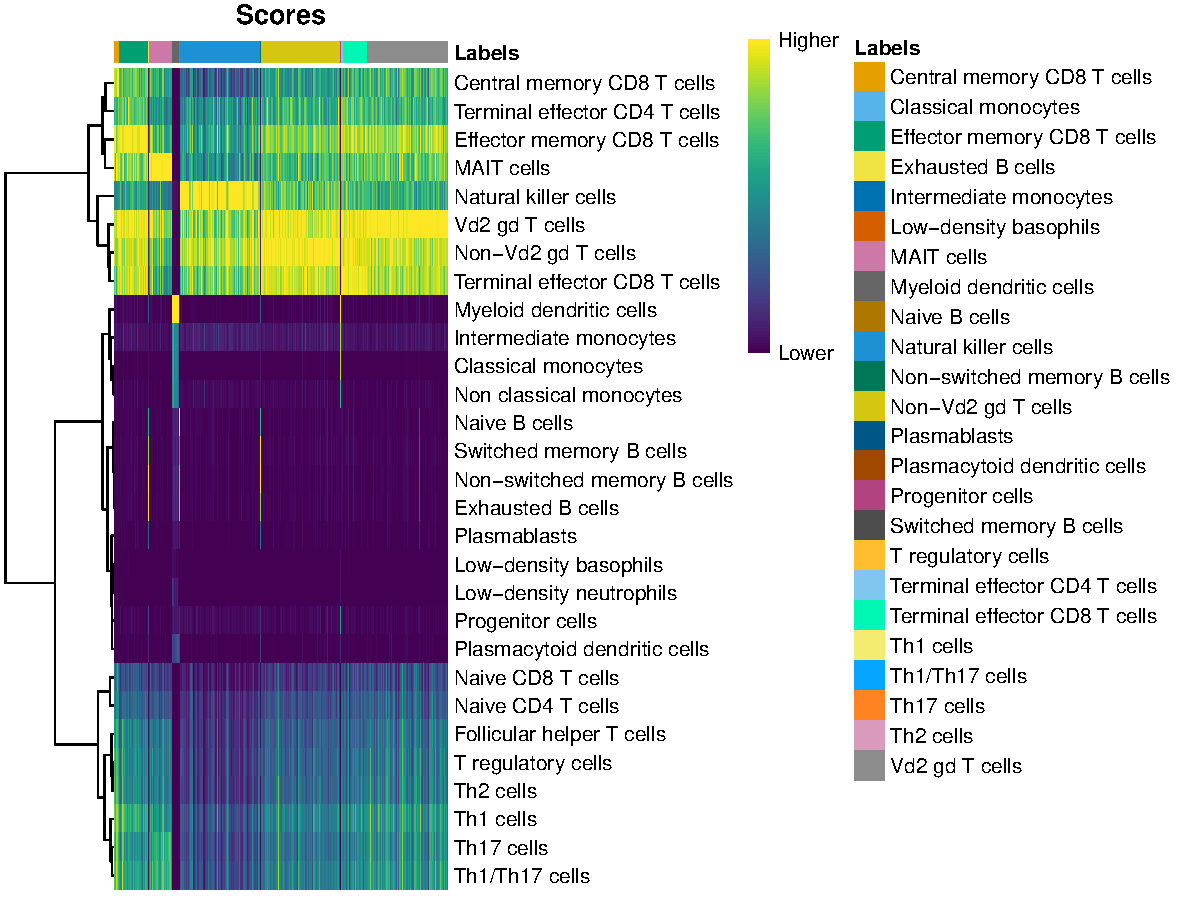
\includegraphics{2-Lett-data-SingleR_pdf_files/figure-pdf/unnamed-chunk-6-1.pdf}

}

\end{figure}

Now these scores are plotted on heatmap and we see a small MAIT portion
annotated

\begin{Shaded}
\begin{Highlighting}[]
\FunctionTok{plotDeltaDistribution}\NormalTok{(pred)}
\end{Highlighting}
\end{Shaded}

\begin{figure}[H]

{\centering 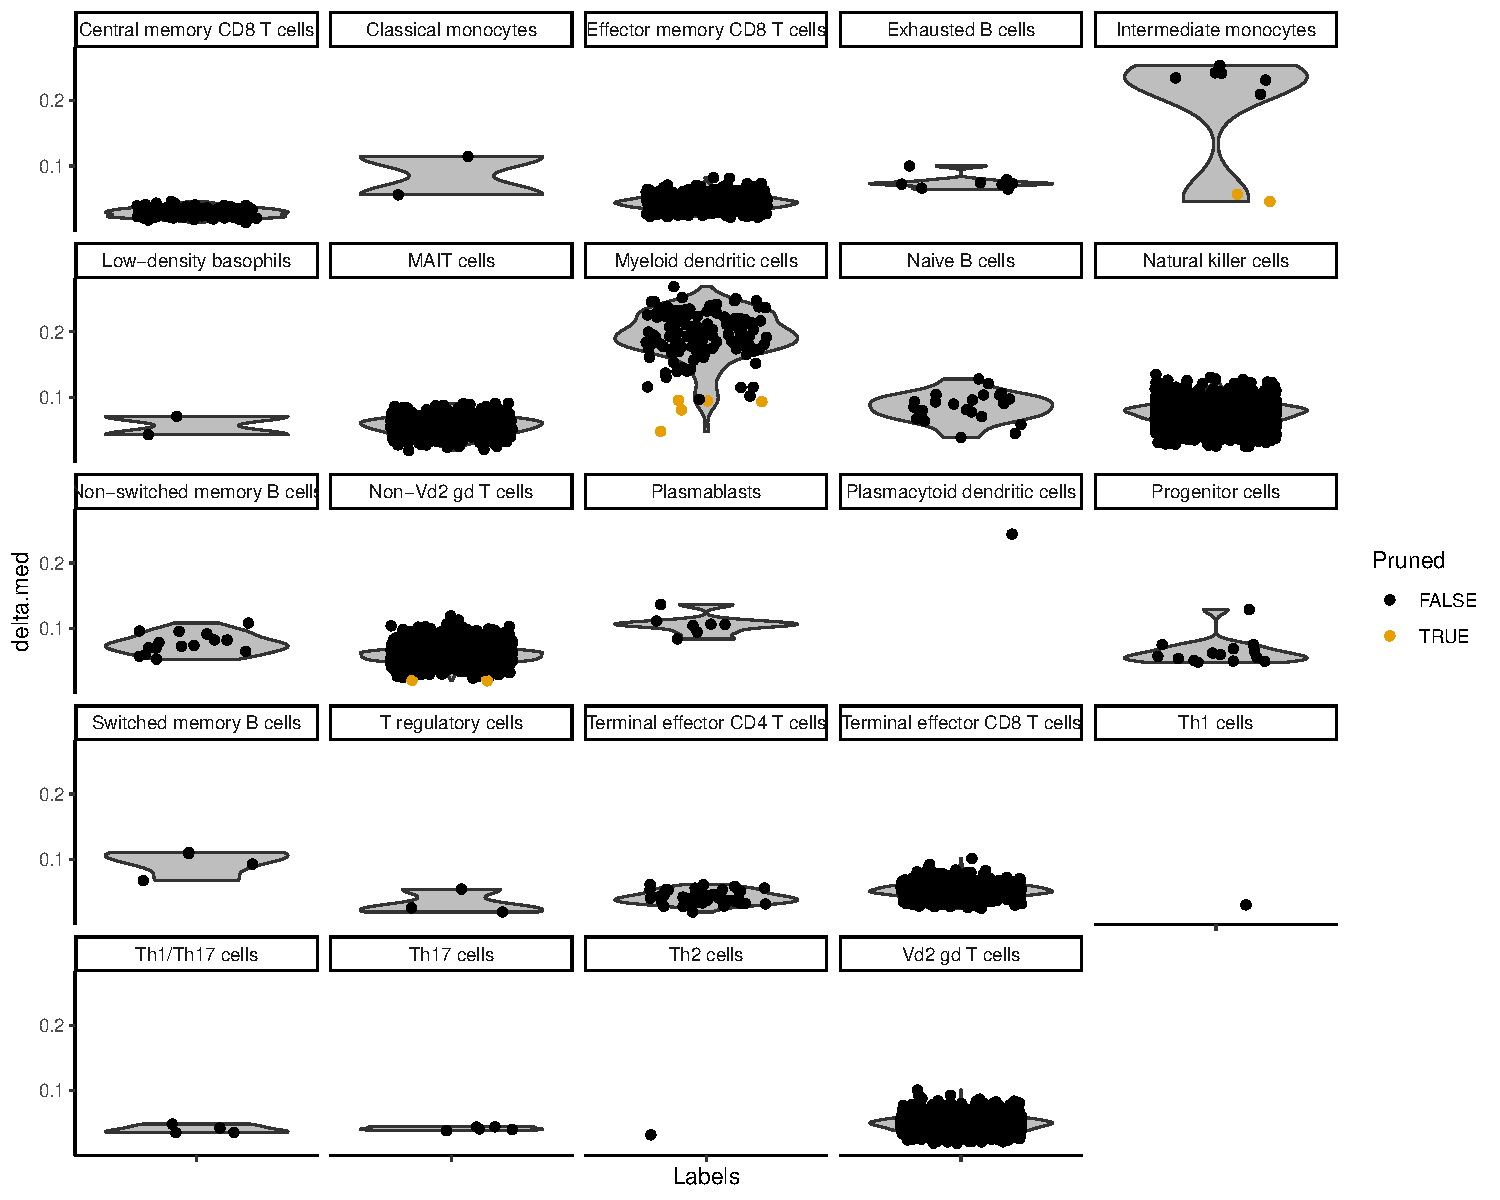
\includegraphics{2-Lett-data-SingleR_pdf_files/figure-pdf/unnamed-chunk-7-1.pdf}

}

\end{figure}

This complex graph shows the rate of false-positives. Nothing important
to mention so far.

\hypertarget{we-make-the-projection-of-all-monacoimmunedata-cell-types-on-lett-dataset}{%
\subsubsection{We make the projection of all MonacoImmuneData cell types
on Lett
dataset}\label{we-make-the-projection-of-all-monacoimmunedata-cell-types-on-lett-dataset}}

UMAP plot showing all 29 fine cell types including MAIT projected on our
dataset. Unfortunately the legend is so small that we can not clearly
see how MAITs are designated

\begin{Shaded}
\begin{Highlighting}[]
\NormalTok{lett.sce}\SpecialCharTok{$}\NormalTok{singleR.labels.fine }\OtherTok{\textless{}{-}}\NormalTok{ pred}\SpecialCharTok{$}\NormalTok{labels[}\FunctionTok{match}\NormalTok{(}\FunctionTok{rownames}\NormalTok{(lett.sce}\SpecialCharTok{@}\NormalTok{colData),}
\FunctionTok{rownames}\NormalTok{(pred))] }

\FunctionTok{plotUMAP}\NormalTok{(lett.sce, }\AttributeTok{colour\_by =} \StringTok{\textquotesingle{}singleR.labels.fine\textquotesingle{}}\NormalTok{,}
\AttributeTok{point\_size =} \FloatTok{1.0}\NormalTok{)}
\end{Highlighting}
\end{Shaded}

\begin{figure}[H]

{\centering 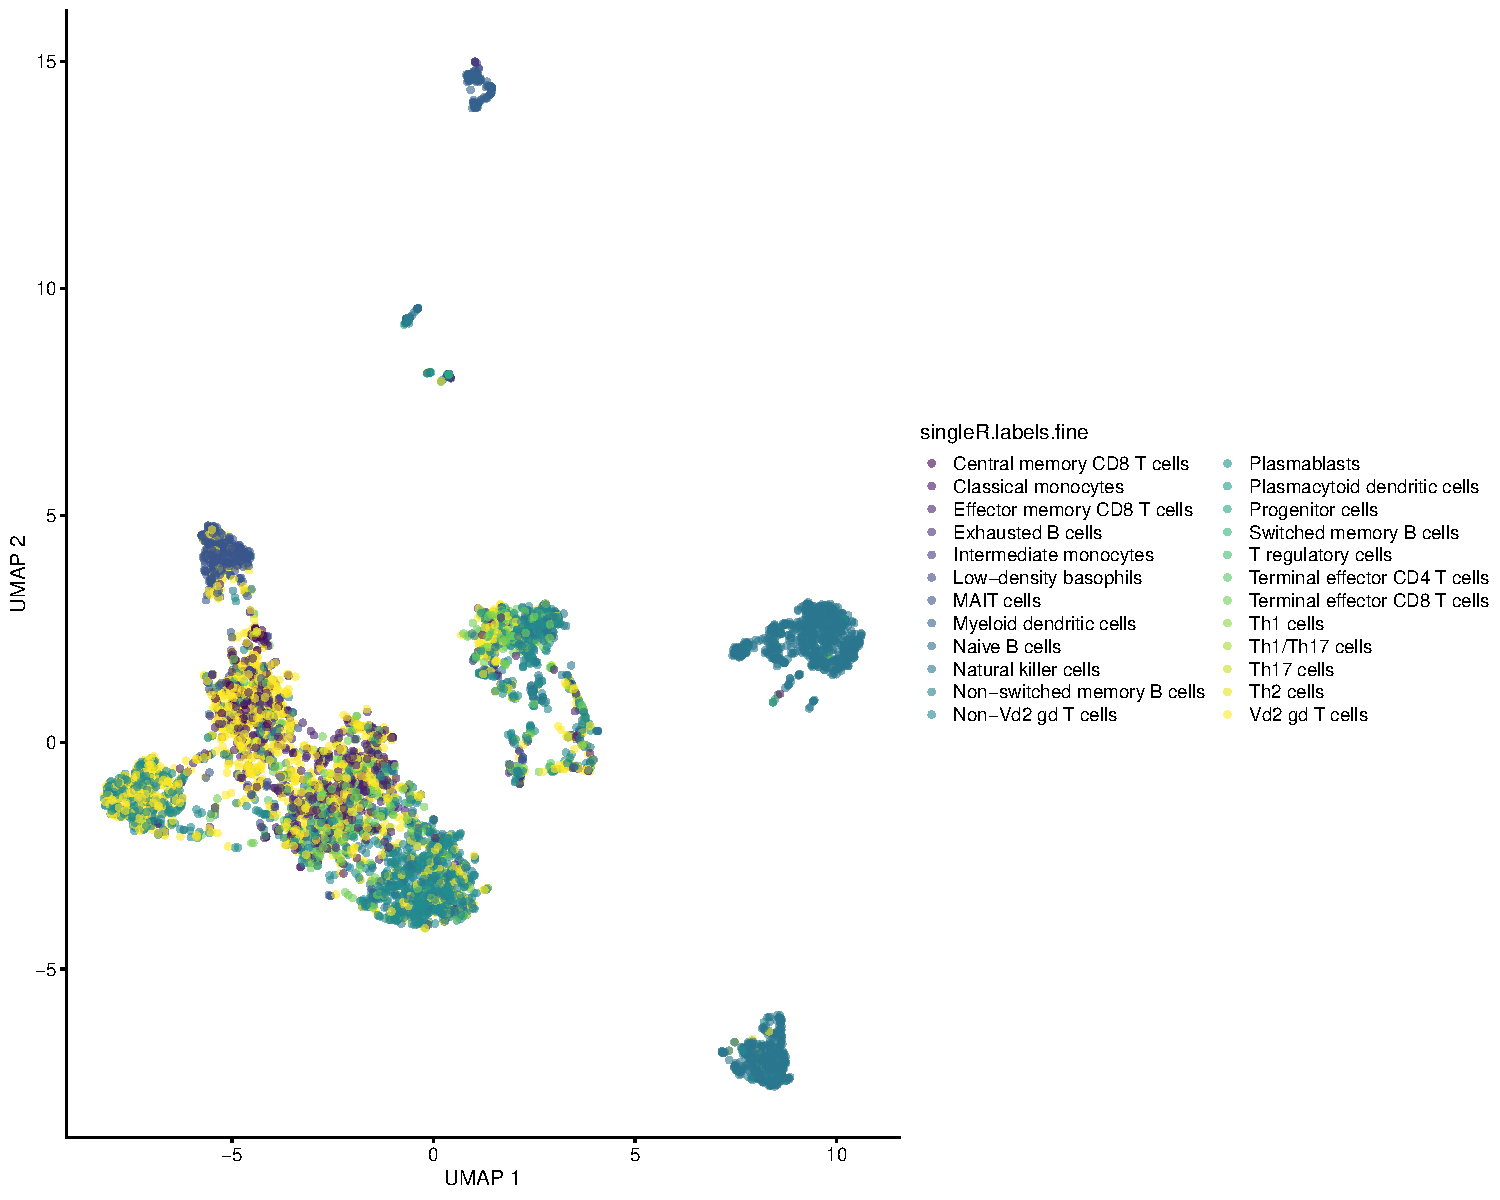
\includegraphics{2-Lett-data-SingleR_pdf_files/figure-pdf/unnamed-chunk-8-1.pdf}

}

\end{figure}

That is why we will produce additional plots below.

\begin{Shaded}
\begin{Highlighting}[]
\NormalTok{tab }\OtherTok{\textless{}{-}} \FunctionTok{table}\NormalTok{(}\AttributeTok{Assigned=}\NormalTok{pred}\SpecialCharTok{$}\NormalTok{labels, }\AttributeTok{Clusters=}\NormalTok{lett.sce}\SpecialCharTok{$}\NormalTok{cellReferences\_celldex\_MonacoImmuneData) }

\FunctionTok{pheatmap}\NormalTok{(}\FunctionTok{log10}\NormalTok{(tab}\SpecialCharTok{+}\DecValTok{10}\NormalTok{), }\AttributeTok{color =} \FunctionTok{colorRampPalette}\NormalTok{(}\FunctionTok{c}\NormalTok{(}\StringTok{\textquotesingle{}white\textquotesingle{}}\NormalTok{,}\StringTok{\textquotesingle{}blue\textquotesingle{}}\NormalTok{))(}\DecValTok{10}\NormalTok{))}
\end{Highlighting}
\end{Shaded}

\begin{figure}[H]

{\centering 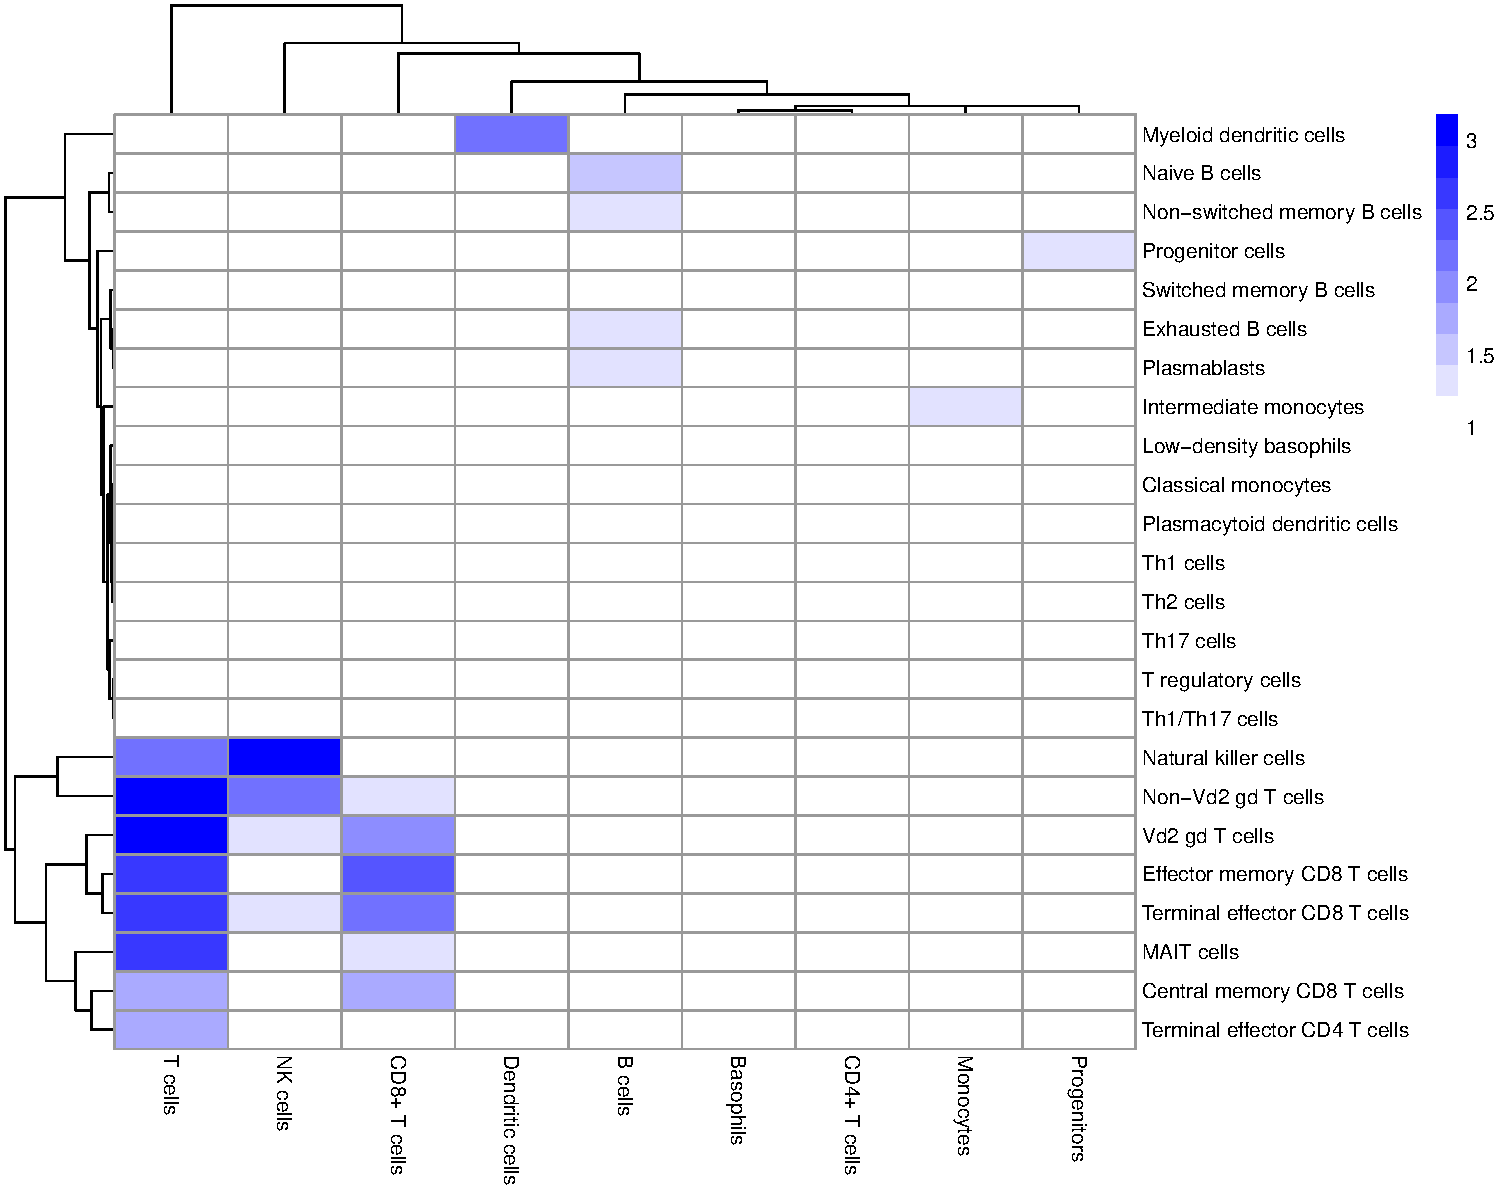
\includegraphics{2-Lett-data-SingleR_pdf_files/figure-pdf/unnamed-chunk-9-1.pdf}

}

\end{figure}

This is another ``heatmap'' showing the relation of MonacoImmuneData
main clusters already contained in the analysis (done by R. Ivanek) and
the newly projected detailed labels. We can see that MAIT cells land
somewhere within T cell cluster together with many other T cell subtypes

\hypertarget{next-we-want-to-do-some-adjusted-vusualizations-to-focus-only-on-mait-cells}{%
\subsubsection{Next we want to do some adjusted vusualizations to focus
only on MAIT
cells}\label{next-we-want-to-do-some-adjusted-vusualizations-to-focus-only-on-mait-cells}}

We use ifelse function to create a new label with only MAIT cells and
``others'' and plot we plot it

\begin{Shaded}
\begin{Highlighting}[]
\NormalTok{cell\_type\_of\_interest }\OtherTok{\textless{}{-}} \StringTok{"MAIT cells"}

\NormalTok{MAIT\_cells }\OtherTok{\textless{}{-}} \FunctionTok{ifelse}\NormalTok{(lett.sce}\SpecialCharTok{@}\NormalTok{colData}\SpecialCharTok{@}\NormalTok{listData[[}\StringTok{"singleR.labels.fine"}\NormalTok{]] }\SpecialCharTok{==} \StringTok{"MAIT cells"}\NormalTok{, }\StringTok{"MAIT cells"}\NormalTok{, }\StringTok{"All other"}\NormalTok{)}

\FunctionTok{colData}\NormalTok{(lett.sce)}\SpecialCharTok{$}\NormalTok{MAIT\_cells }\OtherTok{\textless{}{-}} \FunctionTok{factor}\NormalTok{(MAIT\_cells)}

\NormalTok{colors }\OtherTok{\textless{}{-}} \FunctionTok{c}\NormalTok{(}\StringTok{"MAIT cells"} \OtherTok{=} \StringTok{"red"}\NormalTok{, }\StringTok{"All other"} \OtherTok{=} \StringTok{"lightgrey"}\NormalTok{)}

\NormalTok{p }\OtherTok{\textless{}{-}} \FunctionTok{plotReducedDim}\NormalTok{(lett.sce, }\StringTok{"UMAP"}\NormalTok{, }\AttributeTok{colour\_by =} \StringTok{"MAIT\_cells"}\NormalTok{, }\AttributeTok{point\_size =} \DecValTok{1}\NormalTok{) }\SpecialCharTok{+} \FunctionTok{scale\_colour\_manual}\NormalTok{(}\AttributeTok{values =}\NormalTok{ colors)}
\end{Highlighting}
\end{Shaded}

\begin{verbatim}
Scale for colour is already present.
Adding another scale for colour, which will replace the existing scale.
\end{verbatim}

\begin{Shaded}
\begin{Highlighting}[]
\FunctionTok{print}\NormalTok{(p)}
\end{Highlighting}
\end{Shaded}

\begin{figure}[H]

{\centering 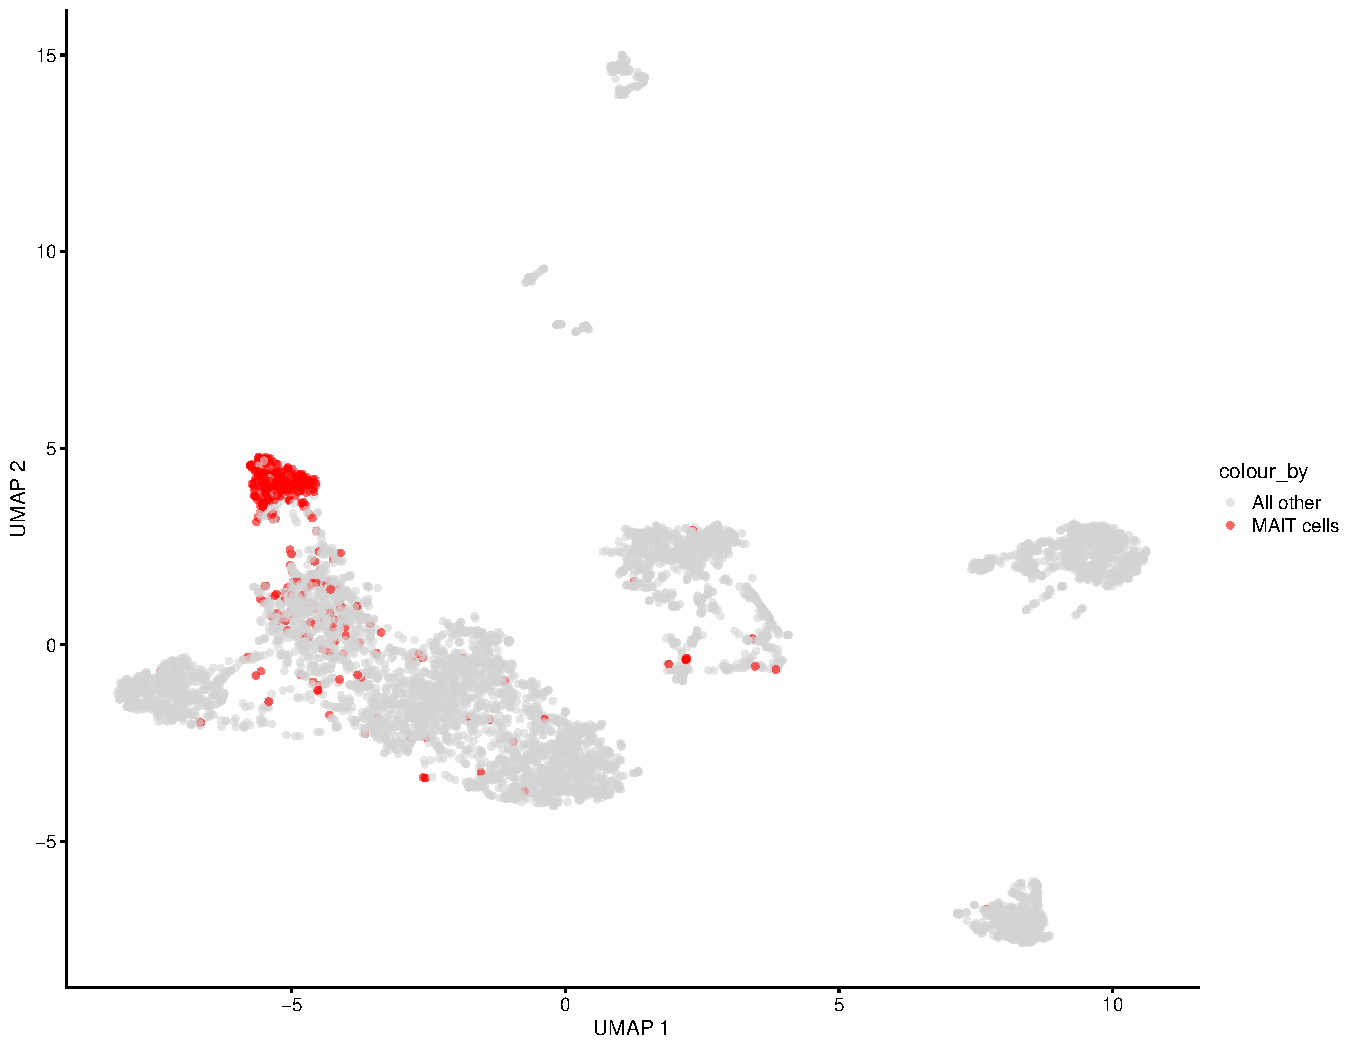
\includegraphics{2-Lett-data-SingleR_pdf_files/figure-pdf/unnamed-chunk-10-1.pdf}

}

\end{figure}

So we see our MAIT cells very nicely among others.

\hypertarget{mait-cell-counts-compared-to-total-t-cells}{%
\subsubsection{MAIT cell counts compared to total T
cells}\label{mait-cell-counts-compared-to-total-t-cells}}

This is achieved by next quite complex code section.

\begin{Shaded}
\begin{Highlighting}[]
\CommentTok{\# Let\textquotesingle{}s count MAIT cells and Other cells}
\NormalTok{MAIT\_cell\_values }\OtherTok{\textless{}{-}} \FunctionTok{colData}\NormalTok{(lett.sce)}\SpecialCharTok{$}\NormalTok{MAIT\_cells}
\NormalTok{value\_counts }\OtherTok{\textless{}{-}} \FunctionTok{table}\NormalTok{(MAIT\_cell\_values)}

\CommentTok{\# now let\textquotesingle{}s annotate all T cells}

\NormalTok{lett.sce}\SpecialCharTok{$}\NormalTok{singleR.labels.main }\OtherTok{\textless{}{-}}\NormalTok{ pred.Tcell}\SpecialCharTok{$}\NormalTok{labels[}\FunctionTok{match}\NormalTok{(}\FunctionTok{rownames}\NormalTok{(lett.sce}\SpecialCharTok{@}\NormalTok{colData),}
\FunctionTok{rownames}\NormalTok{(pred.Tcell))] }

\CommentTok{\# Filtering out only "T cells"}
\NormalTok{t\_cell\_values }\OtherTok{\textless{}{-}}\NormalTok{ lett.sce}\SpecialCharTok{$}\NormalTok{singleR.labels.main}
\NormalTok{is\_t\_cell }\OtherTok{\textless{}{-}}\NormalTok{ t\_cell\_values }\SpecialCharTok{==} \StringTok{"T cells"}
\NormalTok{t\_cell\_counts }\OtherTok{\textless{}{-}} \FunctionTok{sum}\NormalTok{(is\_t\_cell)  }\CommentTok{\# Count the number of "T cells"}
\NormalTok{percent1 }\OtherTok{\textless{}{-}} \FunctionTok{round}\NormalTok{((value\_counts[}\DecValTok{2}\NormalTok{] }\SpecialCharTok{/}\NormalTok{t\_cell\_counts }\SpecialCharTok{*} \DecValTok{100}\NormalTok{),}\DecValTok{1}\NormalTok{)}

\FunctionTok{message}\NormalTok{(}\StringTok{"Number of MAIT cells equals "}\NormalTok{, value\_counts[}\DecValTok{2}\NormalTok{])}
\end{Highlighting}
\end{Shaded}

\begin{verbatim}
Number of MAIT cells equals 459
\end{verbatim}

\begin{Shaded}
\begin{Highlighting}[]
\FunctionTok{message}\NormalTok{(}\StringTok{"Number of all T cells equals "}\NormalTok{, t\_cell\_counts)}
\end{Highlighting}
\end{Shaded}

\begin{verbatim}
Number of all T cells equals 4375
\end{verbatim}

\begin{Shaded}
\begin{Highlighting}[]
\FunctionTok{message}\NormalTok{(}\StringTok{"Persentage of MAIT cells out of all T cells found with this method of annotation equals "}\NormalTok{, percent1)}
\end{Highlighting}
\end{Shaded}

\begin{verbatim}
Persentage of MAIT cells out of all T cells found with this method of annotation equals 10.5
\end{verbatim}

\hypertarget{conclusion-10.5-mait-cells-out-of-all-t-cells-in-liver}{%
\subsubsection{Conclusion: 10.5 MAIT cells out of all T cells in
liver}\label{conclusion-10.5-mait-cells-out-of-all-t-cells-in-liver}}

\hypertarget{analysis-with-singler-and-garner-et-al.-reference}{%
\section{Analysis with SingleR and Garner et
al.~reference}\label{analysis-with-singler-and-garner-et-al.-reference}}

Let's load the new reference data which we saved from previous Seurat
analysis

\begin{Shaded}
\begin{Highlighting}[]
\NormalTok{ref2 }\OtherTok{=} \FunctionTok{readRDS}\NormalTok{(}\StringTok{"output/Garner.seurat.2exp.liver.mait\_analyzed.rds"}\NormalTok{)}
\end{Highlighting}
\end{Shaded}

This command would be needed to convert reference from Seurat to SCE,
but we can avoid it

\begin{Shaded}
\begin{Highlighting}[]
\CommentTok{\#sceasy::convertFormat(Gar.sce,}
  \CommentTok{\# from = "seurat", to = "sce",}
  \CommentTok{\# outFile = "Gar\_sce.rds")}
\CommentTok{\# Gar\_sce is garner.liver.withTrm converted into sce}
\CommentTok{\# Gar.sce \textless{}{-} readRDS("Gar\_sce.rds")}
\CommentTok{\# Gar.sce}
\end{Highlighting}
\end{Shaded}

\hypertarget{extract-count-matrix-from-seurat-object-for-ref-data-and-adjust-both-query-and-reference}{%
\subsubsection{Extract count matrix from Seurat object for ref data and
adjust both query and
reference}\label{extract-count-matrix-from-seurat-object-for-ref-data-and-adjust-both-query-and-reference}}

\begin{Shaded}
\begin{Highlighting}[]
\NormalTok{ref2.counts }\OtherTok{\textless{}{-}}  \FunctionTok{GetAssayData}\NormalTok{(ref2, }\AttributeTok{layer =} \StringTok{"data"}\NormalTok{)}

\NormalTok{common\_genes }\OtherTok{\textless{}{-}} \FunctionTok{intersect}\NormalTok{(}\FunctionTok{rownames}\NormalTok{(lett.sce), }\FunctionTok{rownames}\NormalTok{(ref2))}
\FunctionTok{length}\NormalTok{(common\_genes)}
\end{Highlighting}
\end{Shaded}

\begin{verbatim}
[1] 15243
\end{verbatim}

\begin{Shaded}
\begin{Highlighting}[]
\CommentTok{\# Subset lett.sce to include only common genes}
\NormalTok{lett.sce }\OtherTok{\textless{}{-}}\NormalTok{ lett.sce[common\_genes, ]}

\NormalTok{ref2 }\OtherTok{\textless{}{-}}\NormalTok{ ref2[common\_genes, ]}
\NormalTok{ref2}
\end{Highlighting}
\end{Shaded}

\begin{verbatim}
An object of class Seurat 
15243 features across 17069 samples within 1 assay 
Active assay: RNA (15243 features, 1717 variable features)
 3 layers present: counts, data, scale.data
 2 dimensional reductions calculated: pca, umap
\end{verbatim}

\begin{Shaded}
\begin{Highlighting}[]
\NormalTok{query }\OtherTok{\textless{}{-}} \FunctionTok{assay}\NormalTok{(lett.sce)}
\end{Highlighting}
\end{Shaded}

\hypertarget{lets-construct-reference-object-from-garner-dataset}{%
\subsubsection{Let's construct reference object from Garner
dataset}\label{lets-construct-reference-object-from-garner-dataset}}

\begin{Shaded}
\begin{Highlighting}[]
\NormalTok{cell\_metadata }\OtherTok{\textless{}{-}}\NormalTok{ ref2}\SpecialCharTok{$}\NormalTok{cell\_type}

\NormalTok{metadata\_df }\OtherTok{\textless{}{-}} \FunctionTok{DataFrame}\NormalTok{(}\AttributeTok{cell\_type =}\NormalTok{ cell\_metadata)}

\NormalTok{ref\_se\_object }\OtherTok{\textless{}{-}} \FunctionTok{SummarizedExperiment}\NormalTok{(}\AttributeTok{assays =}\NormalTok{ ref2.counts,}
                                  \AttributeTok{colData =}\NormalTok{ cell\_metadata)}

\NormalTok{ref\_se\_object}\SpecialCharTok{$}\NormalTok{cell\_type }\OtherTok{\textless{}{-}}\NormalTok{ ref\_se\_object}\SpecialCharTok{$}\NormalTok{X}

\NormalTok{ref\_se\_object}\SpecialCharTok{@}\NormalTok{assays}\SpecialCharTok{@}\NormalTok{data}\SpecialCharTok{@}\NormalTok{listData[[}\StringTok{"logcounts"}\NormalTok{]] }\OtherTok{\textless{}{-}}\NormalTok{ ref\_se\_object}\SpecialCharTok{@}\NormalTok{assays}\SpecialCharTok{@}\NormalTok{data}\SpecialCharTok{@}\NormalTok{listData[[}\DecValTok{1}\NormalTok{]]}

\NormalTok{ref\_se\_object}
\end{Highlighting}
\end{Shaded}

\begin{verbatim}
class: SummarizedExperiment 
dim: 19289 17069 
metadata(0):
assays(2): '' logcounts
rownames(19289): AL627309.1 FAM87B ... AC233755.1 AC240274.1
rowData names(0):
colnames(17069): 1_AAAGATGAGTTGAGAT 1_AAATGCCGTGCTCTTC ...
  8_TTTGTCAGTGCATCTA 8_TTTGTCATCTTAGAGC
colData names(2): X cell_type
\end{verbatim}

\hypertarget{we-make-second-mait-annotation-prediction-model-based-on-garner-reference}{%
\subsubsection{We make second MAIT annotation prediction model based on
Garner
reference}\label{we-make-second-mait-annotation-prediction-model-based-on-garner-reference}}

\begin{Shaded}
\begin{Highlighting}[]
\NormalTok{pred2 }\OtherTok{\textless{}{-}} \FunctionTok{SingleR}\NormalTok{(}\AttributeTok{test =}\NormalTok{ query, }\AttributeTok{ref =}\NormalTok{ ref\_se\_object, }\AttributeTok{labels =}\NormalTok{ ref\_se\_object}\SpecialCharTok{$}\NormalTok{cell\_type)}
\end{Highlighting}
\end{Shaded}

\hypertarget{annotation-qc-plots}{%
\subsubsection{Annotation ``QC'' plots}\label{annotation-qc-plots}}

We see here that MAIT are annotated with very high score, and there is
minimal similarity between Tmem and MAIT in our dataset. But ``Other''
cells have significant similarity with both MAIT and Tmem

\begin{Shaded}
\begin{Highlighting}[]
\FunctionTok{plotScoreHeatmap}\NormalTok{(pred2)}
\end{Highlighting}
\end{Shaded}

\begin{figure}[H]

{\centering 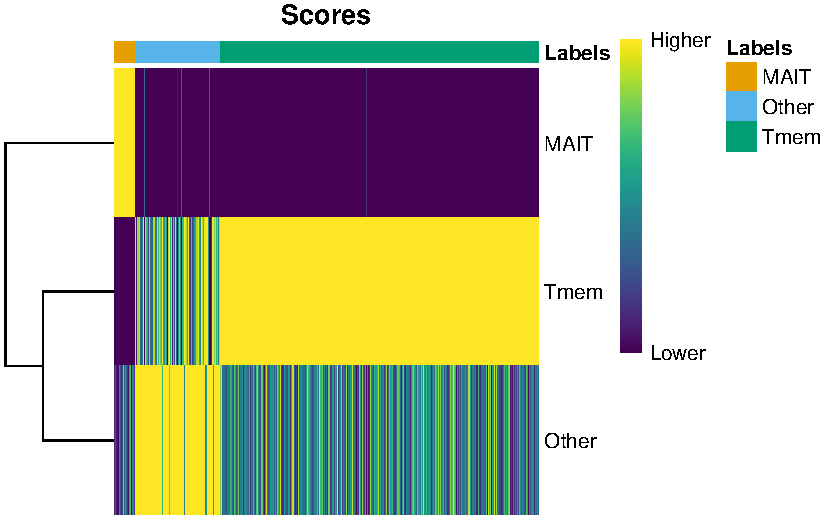
\includegraphics{2-Lett-data-SingleR_pdf_files/figure-pdf/unnamed-chunk-17-1.pdf}

}

\end{figure}

There seems to be no false positives

\begin{Shaded}
\begin{Highlighting}[]
\FunctionTok{plotDeltaDistribution}\NormalTok{(pred2)}
\end{Highlighting}
\end{Shaded}

\begin{figure}[H]

{\centering 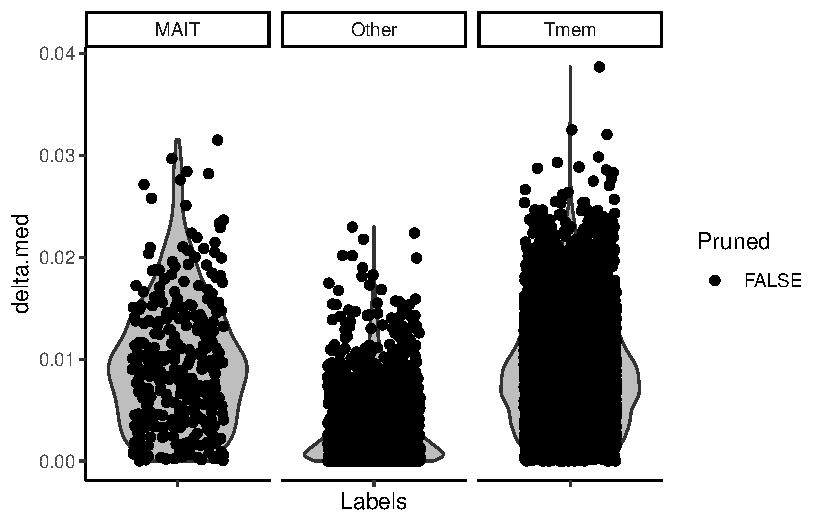
\includegraphics{2-Lett-data-SingleR_pdf_files/figure-pdf/unnamed-chunk-18-1.pdf}

}

\end{figure}

\hypertarget{we-make-umap-projection-of-garner-et-al.-cell-types-on-lett-dataset}{%
\subsubsection{We make UMAP projection of Garner et al.~cell types on
Lett
dataset}\label{we-make-umap-projection-of-garner-et-al.-cell-types-on-lett-dataset}}

It looks simple. We see MAIT likely in the same position as in previous
projection model, but they seem to be a little bit less now

\begin{Shaded}
\begin{Highlighting}[]
\NormalTok{lett.sce}\SpecialCharTok{$}\NormalTok{label.Garner }\OtherTok{\textless{}{-}}\NormalTok{ pred2}\SpecialCharTok{$}\NormalTok{labels[}\FunctionTok{match}\NormalTok{(}\FunctionTok{rownames}\NormalTok{(lett.sce}\SpecialCharTok{@}\NormalTok{colData), }\FunctionTok{rownames}\NormalTok{(pred2))] }

\FunctionTok{plotUMAP}\NormalTok{(lett.sce, }\AttributeTok{colour\_by =} \StringTok{\textquotesingle{}label.Garner\textquotesingle{}}\NormalTok{,}\AttributeTok{point\_size =} \FloatTok{1.0}\NormalTok{)}
\end{Highlighting}
\end{Shaded}

\begin{figure}[H]

{\centering 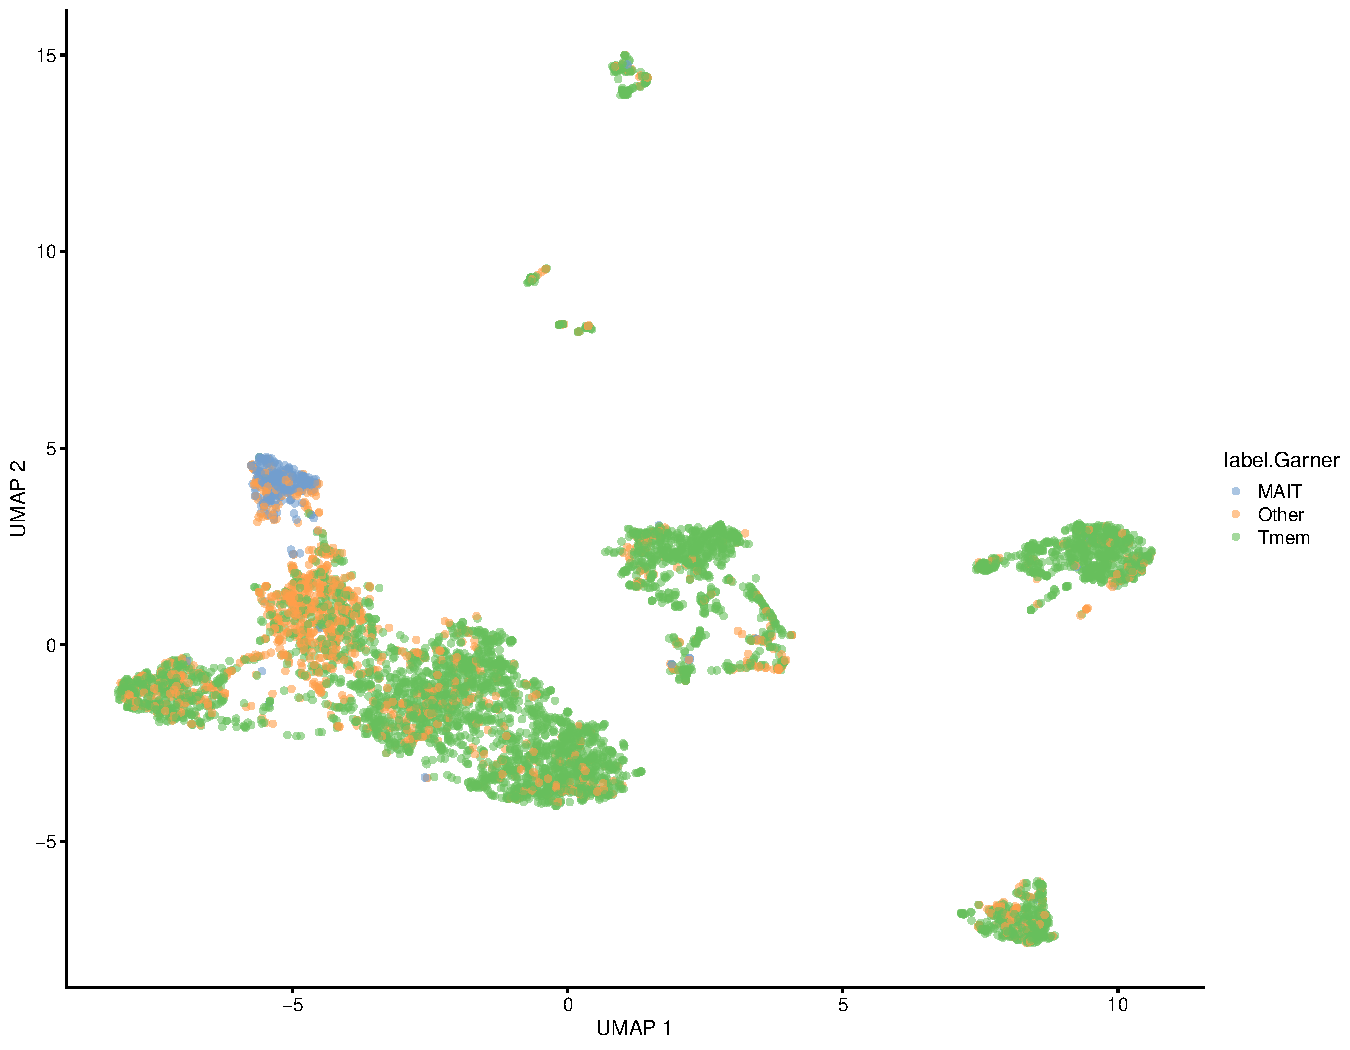
\includegraphics{2-Lett-data-SingleR_pdf_files/figure-pdf/unnamed-chunk-19-1.pdf}

}

\end{figure}

We use ifelse function to create new labels with only MAIT label and
``others''

\begin{Shaded}
\begin{Highlighting}[]
\CommentTok{\#cell\_type\_of\_interest \textless{}{-} "MAIT cells"}

\NormalTok{MAIT\_cells }\OtherTok{\textless{}{-}} \FunctionTok{ifelse}\NormalTok{(lett.sce}\SpecialCharTok{@}\NormalTok{colData}\SpecialCharTok{@}\NormalTok{listData[[}\StringTok{"label.Garner"}\NormalTok{]] }\SpecialCharTok{==} \StringTok{"MAIT"}\NormalTok{, }\StringTok{"MAIT"}\NormalTok{, }\StringTok{"All other"}\NormalTok{)}

\FunctionTok{colData}\NormalTok{(lett.sce)}\SpecialCharTok{$}\NormalTok{MAIT\_cells\_Garner }\OtherTok{\textless{}{-}} \FunctionTok{factor}\NormalTok{(MAIT\_cells)}

\NormalTok{colors }\OtherTok{\textless{}{-}} \FunctionTok{c}\NormalTok{(}\StringTok{"MAIT"} \OtherTok{=} \StringTok{"red"}\NormalTok{, }\StringTok{"All other"} \OtherTok{=} \StringTok{"lightgrey"}\NormalTok{)}

\NormalTok{p2 }\OtherTok{\textless{}{-}} \FunctionTok{plotReducedDim}\NormalTok{(lett.sce, }\StringTok{"UMAP"}\NormalTok{, }\AttributeTok{colour\_by =} \StringTok{"MAIT\_cells\_Garner"}\NormalTok{, }\AttributeTok{point\_size =} \DecValTok{1}\NormalTok{) }\SpecialCharTok{+} \FunctionTok{scale\_colour\_manual}\NormalTok{(}\AttributeTok{values =}\NormalTok{ colors)}
\end{Highlighting}
\end{Shaded}

\begin{verbatim}
Scale for colour is already present.
Adding another scale for colour, which will replace the existing scale.
\end{verbatim}

\begin{Shaded}
\begin{Highlighting}[]
\FunctionTok{print}\NormalTok{(p2)}
\end{Highlighting}
\end{Shaded}

\begin{figure}[H]

{\centering 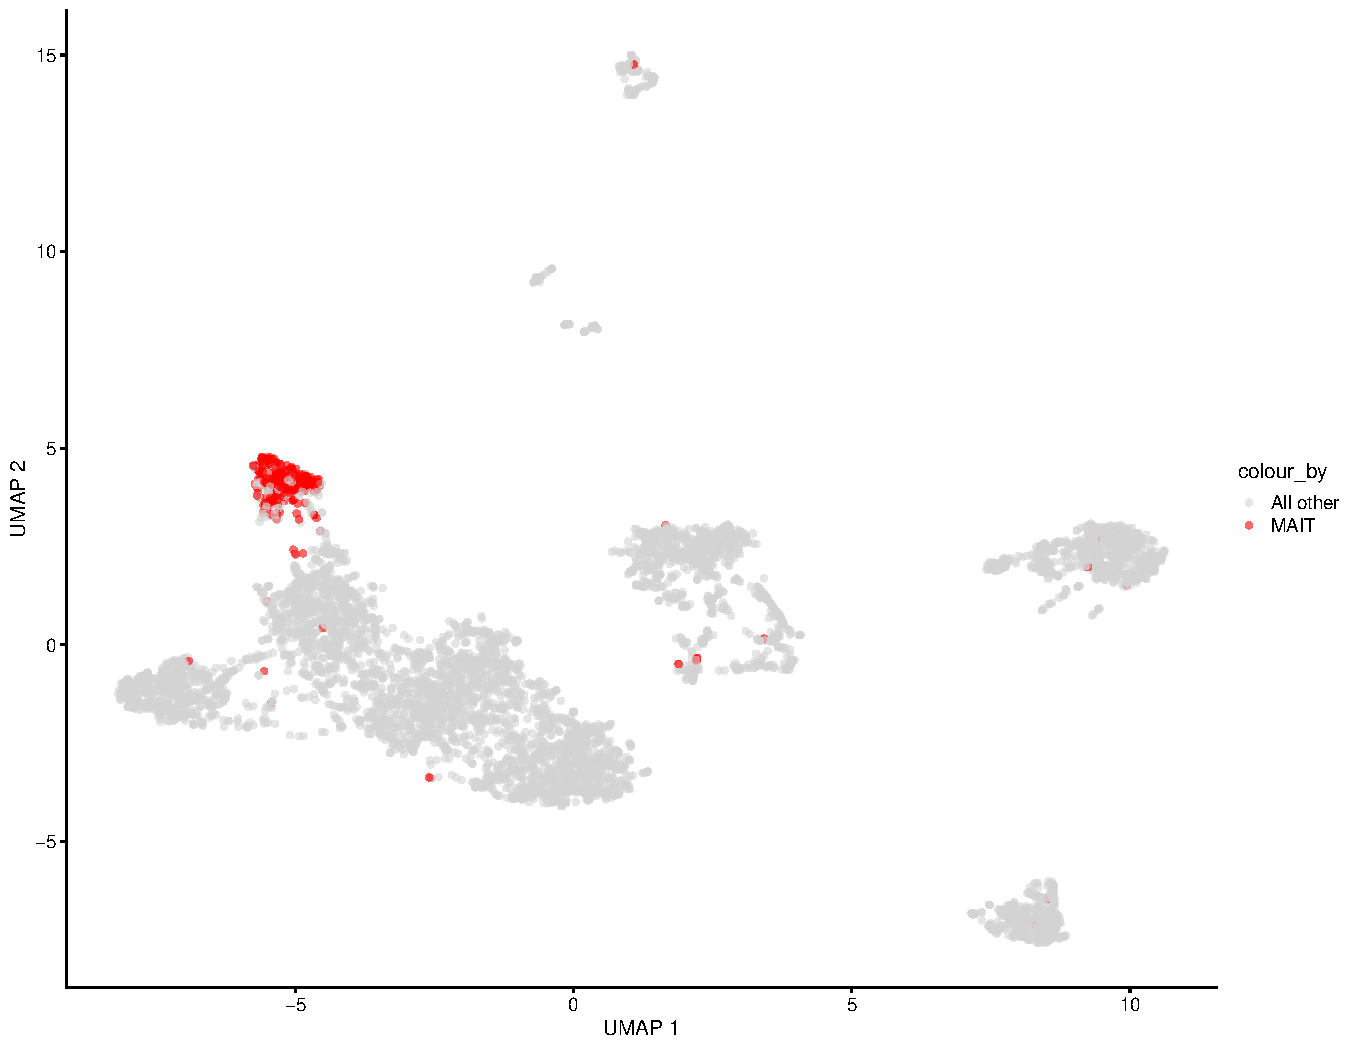
\includegraphics{2-Lett-data-SingleR_pdf_files/figure-pdf/unnamed-chunk-20-1.pdf}

}

\end{figure}

\hypertarget{calculating-mait-cell-number-and-ratio-to-all-t-cells}{%
\subsubsection{Calculating MAIT cell number and ratio to all T
cells}\label{calculating-mait-cell-number-and-ratio-to-all-t-cells}}

\begin{Shaded}
\begin{Highlighting}[]
\NormalTok{MAIT\_cell\_values2 }\OtherTok{\textless{}{-}} \FunctionTok{colData}\NormalTok{(lett.sce)}\SpecialCharTok{$}\NormalTok{MAIT\_cells\_Garner}
\NormalTok{value\_counts2 }\OtherTok{\textless{}{-}} \FunctionTok{table}\NormalTok{(MAIT\_cell\_values2)}
\NormalTok{percent2 }\OtherTok{\textless{}{-}} \FunctionTok{round}\NormalTok{((value\_counts2[}\DecValTok{2}\NormalTok{] }\SpecialCharTok{/}\NormalTok{t\_cell\_counts }\SpecialCharTok{*} \DecValTok{100}\NormalTok{),}\DecValTok{1}\NormalTok{)}
\FunctionTok{message}\NormalTok{(}\StringTok{"Number of MAIT cells equals "}\NormalTok{, value\_counts2[}\DecValTok{2}\NormalTok{])}
\end{Highlighting}
\end{Shaded}

\begin{verbatim}
Number of MAIT cells equals 324
\end{verbatim}

\begin{Shaded}
\begin{Highlighting}[]
\FunctionTok{message}\NormalTok{(}\StringTok{"Number of all T cells equals "}\NormalTok{, t\_cell\_counts)}
\end{Highlighting}
\end{Shaded}

\begin{verbatim}
Number of all T cells equals 4375
\end{verbatim}

\begin{Shaded}
\begin{Highlighting}[]
\FunctionTok{message}\NormalTok{(}\StringTok{"Persentage of MAIT cells out of all T cells found with this method of annotation equals "}\NormalTok{, percent2)}
\end{Highlighting}
\end{Shaded}

\begin{verbatim}
Persentage of MAIT cells out of all T cells found with this method of annotation equals 7.4
\end{verbatim}

\hypertarget{conclusion}{%
\subsubsection{Conclusion}\label{conclusion}}

It seems that we identified the position of our MAIT cells correctly,
since two independent dataset projections make very similar result.
Using Garner dataset we get slightly less cells identified as MAIT.
There might be different reasons for this. Perhaps, batch effect is one
of them.



\end{document}
